%%%%%%%%%%%%%%%%%%%%%%%%%%%%%%%%%%%%%%%%%%%%%%%%%%%%%%%%%%%%%%%%%%%%%%%%%%%%%%%%
\chapter{Νευρομυοσκελετικό Σύστημα}

Σε αυτό το κεφάλαιο παρουσιάζουμε την διαδικασία της ορθής δυναμικής σε νευρομυοσκελετικά μοντέλα. Στόχος είναι να εκτιμηθούν οι δυνάμεις που παράγονται από τους μύες, οι οποίες μετατρέπονται σε  ροπές, οι οποίες με την σειρά τους σε κίνηση που προήρθε από την νευρική διέγερση των μυών. Η παραπάνω διαδικασία μπορεί να χωριστεί σε τέσσερα βήματα, την μυική ενεργοποίση (\eng{muscle activation dynamics}), την μυική συστολή (\eng{muscle contraction dynamics}), την μυοσκελετική γεωμετρία και τέλος την εξίσωσης της κίνησης, η οποία επιτρέπει την μετατροπή της ροπής των αρθρώσεων σε κίνηση.

%%%%%%%%%%%%%%%%%%%%%%%%%%%%%%%%%%%%%%%%%%%%%%%%%%%%%%%%%%%%%%%%%%%%%%%%%%%%%%%%
\section{H Φυσιολογία του Μυ}

%%%%%%%%%%%%%%%%%%%%%%%%%%%%%%%%%%%%%%%%%%%%%%%%%%%%%%%%%%%%%%%%%%%%%%%%%%%%%%%%
\subsection{Δομή}

Ο σκελετικός μυς είναι μια συλλογή από μυϊκά κύτταρα (μυϊκές ίνες) \cite{zirinoglou}. Ο αριθμός των μυϊκών ινών εξαρτάται από το μέγεθος του μυός και ποικίλει από μερικές εκατοντάδες έως αρκετές χιλιάδες ίνες. Ολόκληρος ο μυς καλύπτεται και προστατεύεται από ένα συνδετικό περιτοναϊκό ιστό ο όποιος περιβάλλει κάθε μυϊκή ίνα, τένοντα, οστό, νεύρο και αγγείο. Ο μυς διαιρείται περεταίρω σε αρκετές μυϊκές δεσμίδες. Κάθε δέσμη περιέχει περίπου εκατό μυϊκές ίνες. Κάθε ίνα έχει διάμετρο 50 με 100μm (χιλιοστά του χιλιοστόμετρου), μήκος 2 με 6 εκατοστά και περιέχει περισσότερα από 1000 με 2000 μυϊκά ινίδια, τα οποία με την σειρά τους περιέχουν μια αλυσίδα από σαρκομέριο. Κάθε μυϊκό ινίδιο αποτελείται από αρκετούς τύπους πρωτεϊνών.

\begin{figure}[H]
    \centering
    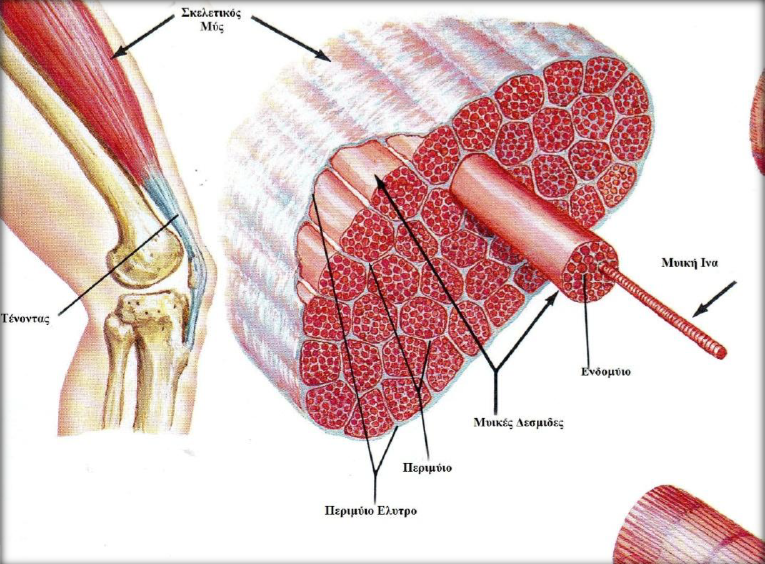
\includegraphics[width=.7\textwidth]{neuromusculoskeletal/fig/muscle-fysiology.png}
    \caption{Σκελετικός Μυς: Ανατομική Περιγραφή (τροποποιημένη από \eng{Netter} 1987)}
    \label{fig:muscle-fysiology}
\end{figure}

\begin{figure}[H]
    \centering
    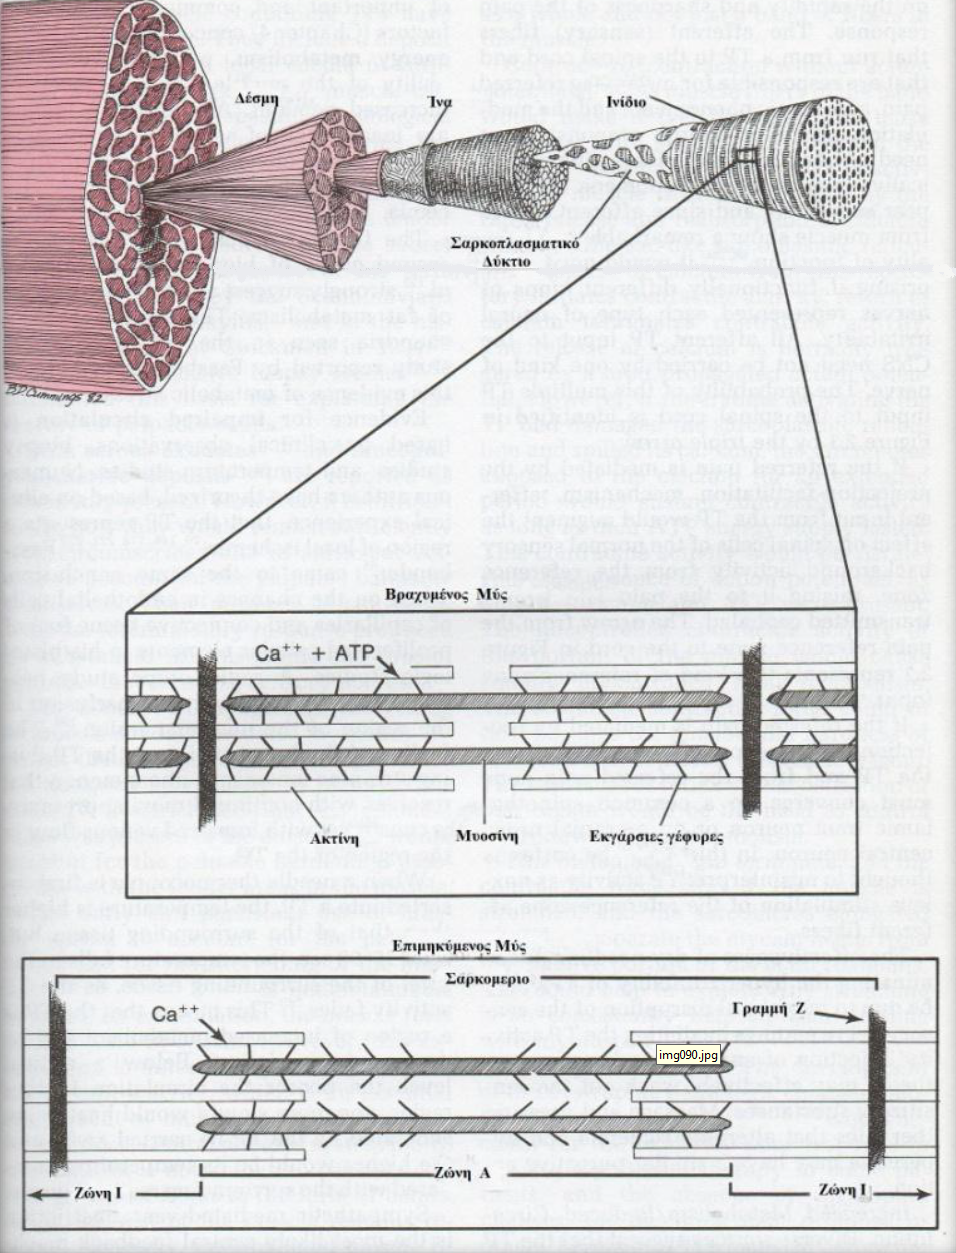
\includegraphics[width=.7\textwidth, height=0.5\textheight]{neuromusculoskeletal/fig/muscle-fysiology2.png}
    \caption{Δομή και συσταλτικός μηχανισμός του φυσιολογικού σκελετικού μυός(από \eng{Travell \& Simons} 1999)}
    \label{fig:muscle-fysiology2}
\end{figure}

Ο μυς διαιρείται περεταίρω σε αρκετές μυϊκές δεσμίδες. Κάθε δέσμη περιέχει περίπου εκατό μυϊκές ίνες. Κάθε ίνα έχει διάμετρο 50 με 100μm (χιλιοστά του χιλιοστόμετρου), μήκος 2 με 6 εκατοστά και περιέχει περισσότερα από 1000 με 2000 μυϊκά ινίδια , τα οποία με την σειρά τους περιέχουν μια αλυσίδα από σαρκομέριο. Κάθε μυϊκό ινίδιο αποτελείται από αρκετούς τύπους πρωτεϊνών.

Τo σαρκομέριο είναι η συσταλτή μονάδα του μυϊκού ινιδίου και αποτελείται από επικαλυπτόμενες εγκάρσιες γέφυρες ακτίνης και μυοσίνης. Το σαρκομέριο δίνει την δυνατότητα στον μυ να συσπάται και να χαλαρώνει. Όταν ο μυς συσπάται, τα λεπτά νημάτια ακτίνης και μυοσίνης ολισθαίνουν μεταξύ τους και ο μυς βραχύνεται. Όταν ο μυς χαλαρώνει, οι εγκάρσιες γέφυρες ολισθαίνουν ήπια και ξεχωριστά, και ο μυς επιστρέφει στο μήκος ηρεμίας.

\begin{figure}[H]
    \centering
    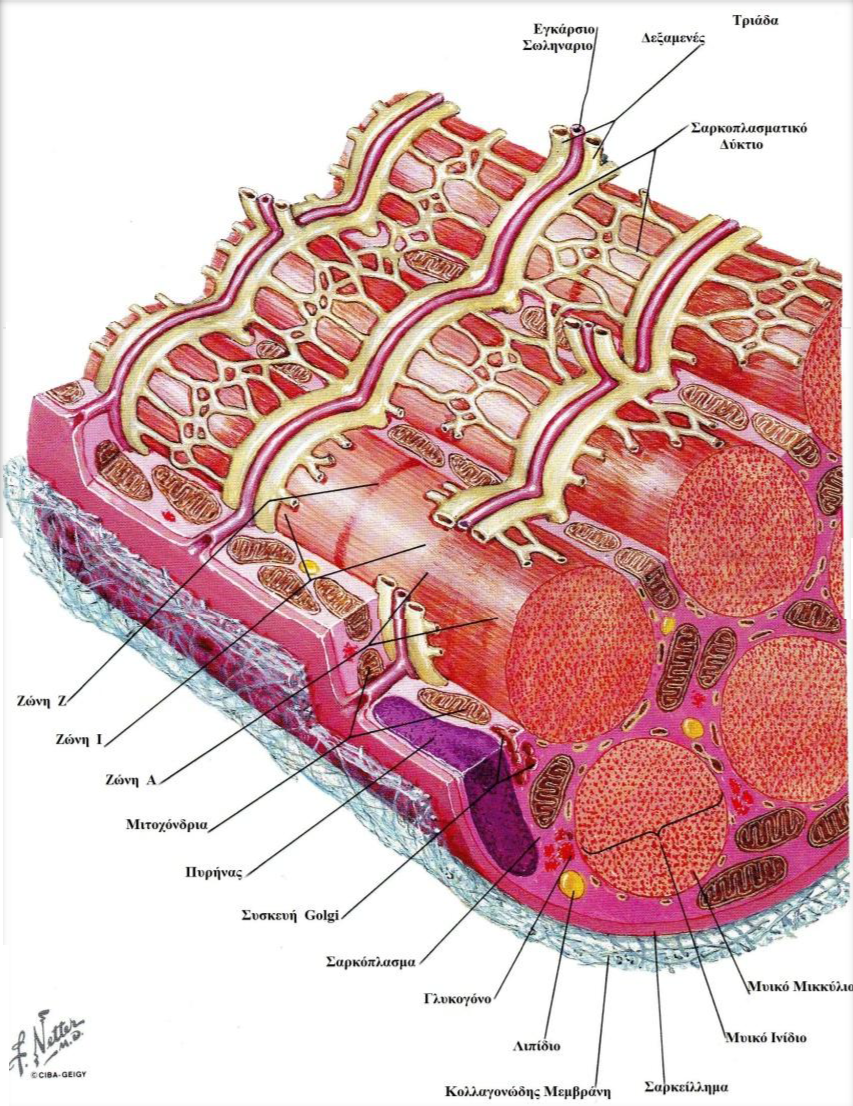
\includegraphics[width=.7\textwidth, height=0.7\textheight]{neuromusculoskeletal/fig/muscle-fysiology3.png}
    \caption{Σαρκοπλασματικό Δίκτυο (τροποποιημένη από \eng{Netter} 1987 )}
    \label{fig:muscle-fysiology3}
\end{figure}

%%%%%%%%%%%%%%%%%%%%%%%%%%%%%%%%%%%%%%%%%%%%%%%%%%%%%%%%%%%%%%%%%%%%%%%%%%%%%%%%
\subsection{Σαρκοπλασματικό Δίκτυο}

Το σαρκοπλασματικό (\eng{Kandel E.et al} 2000, \eng{Fawcett D} 1986) δίκτυο είναι ένα δίκτυο σωληνοειδούς μορφής το οποίο εκτείνεται σε ολόκληρο τον μυ. Τα επιμήκη σαρκοπλασματικό σωληνάρια καταδύονται σε μια σχετικά μεγάλη τελική δεξαμενή σε οποιαδήποτε άκρη του σαρκομερίου. Δυο τελικές δεξαμενές σε συνδυασμό με ένα εγκάρσιο σωληνάριο(\eng{T-tubule}) σχηματίζουν μια τριάδα (\eng{Silverthorn D} 1998). Παρόλο που οι τρεις αυτές δομές έχουν πολύ στενή σχέση μεταξύ τους, δεν γνωρίζουμε να υπάρχει κάποιος συνδετικός μηχανισμός. Η τριάδα είναι τοποθετημένη σε καίρια θέση δίπλα από το τμήμα της μυϊκής ίνας το οποίο παράγει τις απαραίτητες δυνάμεις για την συστολή. Το εγκάρσιο σωληνάριο παίζει ένα σημαντικό ρόλο στη διέλευση του δυναμικού ενέργειας βαθιά μέσα στον μυ. Ο ρόλος του σαρκοπλασματικου δικτύου είναι να αποθηκεύει $Ca^{2+}$, το οποίο είναι απαραίτητο για την συστολή του μυός.

%%%%%%%%%%%%%%%%%%%%%%%%%%%%%%%%%%%%%%%%%%%%%%%%%%%%%%%%%%%%%%%%%%%%%%%%%%%%%%%%
\subsection{Το Νευρικό Σύστημα}

Η κύρια εργασία του κινητικού νευρικού συστήματος είναι να ελέγχει και να συντονίζει τη λειτουργία των συσταλτών στοιχείων σε όλους τους μύες ταυτόχρονα έτσι ώστε να εφαρμόζεται η κατάλληλη τάση στον σκελετό για να παραχθεί η επιθυμητή κίνηση (\eng{Kandel et al} 200).

\begin{figure}[H]
    \centering
    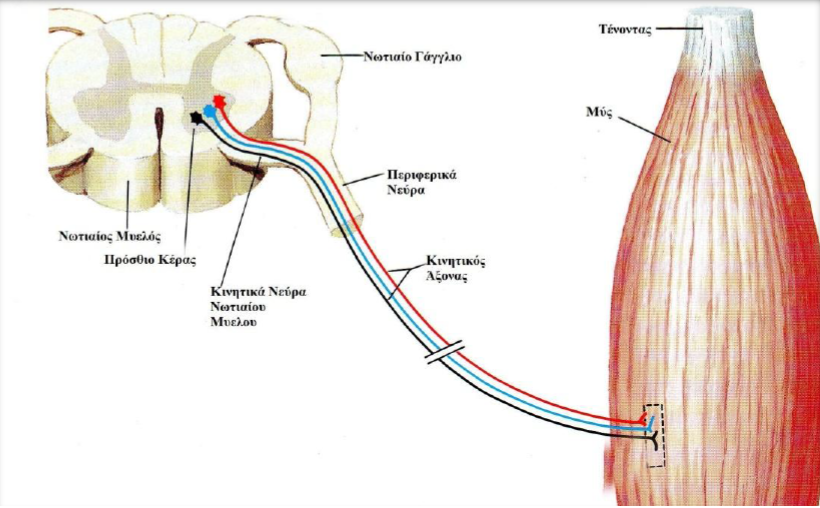
\includegraphics[width=.8\textwidth]{neuromusculoskeletal/fig/muscle-fysiology4.png}
    \caption{Κινητική Μονάδα (τροποποιημένη από \eng{Netter} 1987)}
    \label{fig:muscle-fysiology4}
\end{figure}

Ο κινητικός νευρώνας θεωρείται ως η λειτουργική μονάδα του κινητικού νευρικού συστήματος. Τα κυτταρικά σώματα των κινητικών νευρώνων είναι στοιβαγμένα σε έναν κινητικό πυρήνα μέσα στο κοιλιακό τμήμα της σπονδυλικής στήλης. Ο άξονας κάθε κινητικού νευρώνα εκφύεται από την σπονδυλική στήλη διαμέσου μιας κοιλιακής ρίζας (ή ενός κρανιακού νεύρου από το εγκεφαλικό στέλεχος) και διαιρείται σε μικρότερους κλάδους περιφερικών νεύρων μέχρι να εισέλθει στον μυ που ελέγχεται από αυτό το νεύρο. Όταν ένας μεγάλος εμμύελος κινητικός άξονας πλησιάζει μια μυϊκή ίνα, διαιρείται σε πολλαπλά νευρικά κλώνια τα οποία διατρέχουν μικρές αποστάσεις στην επιφάνεια του μυός, πριν απολήξουν. Η περιοχή μιας μυϊκής ίνας η οποία βρίσκεται κάτω από ένα νευρικό κλωνίο, ονομάζεται τελική κινητική πλάκα.

Οι μυϊκές άτρακτοι βρίσκονται τοποθετημένοι μέσα σε όλους τους μύες του σώματος και θεωρούνται τα πιο σημαντικά ιδιοδεκτικά όργανα. Είναι απαραίτητες για την γνώση της θέσης και της κίνησης των μελών, αλλά επίσης και συντελεστές κλειδιά για τον λεπτό κινητικό Έλενο.

\begin{figure}[H]
    \centering
    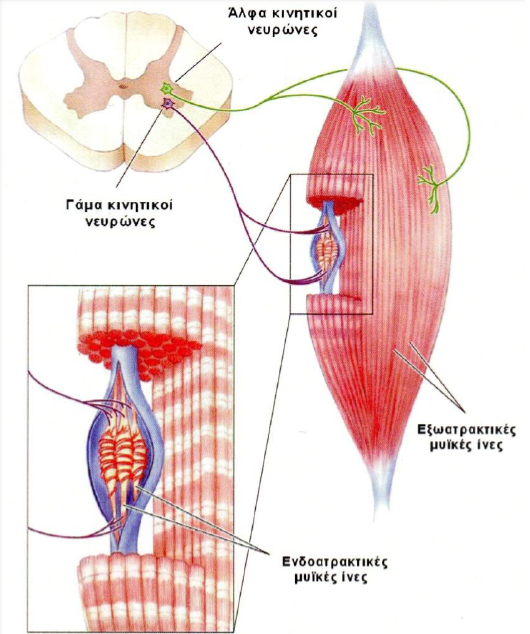
\includegraphics[width=.8\textwidth]{neuromusculoskeletal/fig/muscle-fysiology5.png}
    \caption{Κινητική Μονάδα(Μυϊκή άτρακτος}
    \label{fig:muscle-fysiology5}
\end{figure}

Ο μεγαλύτερος αριθμός των μυϊκών ατράκτων βρίσκεται στο μυϊκό σώμα των σκελετικών μυών και ειδικότερα στους μύες των δάκτυλων, στους εξωφθαλμιους μύες και στους μύες του λαιμού σε αντίθεση με τους μύες που ελέγχουν την αδρή κινητικότητα. Αποτελείται από μικροσκοπικές ενδοατρακτικες γραμμωτές ίνες, οι οποίες βρίσκονται παράλληλα με τις εξωατρακτικες γραμμωτές ίνες. Η μυϊκή άτρακτος καταγράφει την ταχύτητα και την διάρκεια της διάτασης και αντιλαμβάνεται τις αλλαγές του μήκους του μυός. Οι ίνες της μυϊκής ατράκτου αντιλαμβάνονται πόσο γρήγορα διατείνεται ο μυς. Πρωταγωγείς (τύπου Ια) και δευτεραγωγείς (τύπου ΙΙ) κεντρομόλες ίνες ανέρχονται από τις μυϊκές ατράκτους, συνάπτονται με άλφα ή γάμα κινητικούς νευρώνες αντίστοιχα και διευκολύνουν τη σύσπαση των εξωατρακτικων και ενδοατρακτικων ινών.

%%%%%%%%%%%%%%%%%%%%%%%%%%%%%%%%%%%%%%%%%%%%%%%%%%%%%%%%%%%%%%%%%%%%%%%%%%%%%%%%
\subsection{Το Όργανο του ...}%\eng{Golgi}

Το όργανο του \eng{Golgi} βρίσκεται κοντά στην μυοτενόντια σύναψη , τυλίγεται γύρω από τα άκρα των εξωατρακτικων ινών του μυός και είναι ευαίσθητο στην τάση που προκαλείται στον μυ από παθητική διάταση ή από ενεργητική σύσπαση του. Το όργανο του \eng{Golgi} είναι ένας προστατευτικός μηχανισμός που αναστέλλει την σύσπαση του μυός στον όποιο βρίσκεται. Η ουδός πυροδότησης είναι πολύ χαμηλή (ενεργοποιείται εύκολα), μετά από ενεργητική μυϊκή σύσπαση και πολύ υψηλή, μετά από μια παθητική διάταση. Όταν αναπτύσσεται υπερβολική τάση στον μυ, το όργανο του Golgi πυροδοτεί , αναστέλλει τη δραστηριότητα του άλφα κινητικού νευρώνα και μειώνει την τάση του μυός. Κατά την διάρκεια των διαδικασιών της διάτασης , η τάση στον τένοντα καθορίζει αν το κάθε σαρκομέριο του μυός είναι επιμηκυμένο.

Κατά την διάρκεια όμως της ισοτονικής και της ισομετρικής συστολής του μυός η κατάσταση διαφοροποιείται. Ενώ σταματά να διατείνεται η μυϊκή άτρακτος , το τενόντιο όργανο συνεχίζει να βρίσκεται σε διάταση και στην πραγματικότητα ο ρυθμός της πυροδότησης του αυξάνεται σε όλη τη διάρκεια της συστολής. Ο δυναμικός κώδικας του ενάντιου οργάνου σηματοδοτεί το ρυθμό αύξησης της έντασης κατά την διάρκεια της συστολής και το ρυθμό της μείωσης της διέγερσης κατά την διάρκεια της χαλάρωσης .Το πρότυπο διέγερσης των τενόντιων οργάνων κατά την διάρκεια της συστολής δείχνει ότι ο κύριος ρόλος τους είναι να ελέγχουν το ρυθμό της αλλαγής της έντασης σε έναν συστελλόμενο μυ καθώς σηματοδοτούν το ποσό της έντασης που υπάρχει σε έναν ισομετρικά συστελλόμενο μυ. Jim stanev.


%%%%%%%%%%%%%%%%%%%%%%%%%%%%%%%%%%%%%%%%%%%%%%%%%%%%%%%%%%%%%%%%%%%%%%%%%%%%%%%%
\section{Μοντέλο του Μυ}

Ένα μοντέλο του μυ περιγράφει την διαδικασία παραγωγής της δύναμης κάτω από μια νευρική διέγερση και μπορούν να καταταχθούν σε μικροσκοπικά και μακροσκοπικά μοντέλα. Τα μικροσκοπικά μοντέλα ανήκουν στην κατηγορία \eng{Huxley-type} προς τιμή του \eng{Huxley 1957}, ενώ το πιο διάσημο μακροσκοπικό μοντέλο είναι το \eng{Hull-type} προς τιμή του \eng{Hill 1938}. Τα δύο αυτά μοντέλα είναι χρησιμοποιούνται ευρέως στην επιστημονική κοινότητα. Όσον αφορά τα μοντέλα \eng{Hill-type} είναι καταλληλότερα σε εφαρμογές προσομοίωσης, γιατί είναι ποιο απλά και έχουν λιγότερους παραμέτρους που πρέπει να προσδιορισθούν. Για αυτό το λόγο, η ανάλυση που θα γίνει στην συνέχεια αφορά την δεύτερη κατηγορία μοντέλων.

%%%%%%%%%%%%%%%%%%%%%%%%%%%%%%%%%%%%%%%%%%%%%%%%%%%%%%%%%%%%%%%%%%%%%%%%%%%%%%%%
\subsection{Μοντέλο Ενεργοποίησης}

Η αλληλεπίδραση μεταξύ ινιδίων μυοσίνης και ακτίνης ενεργοποιείται όταν το μυϊκό κύτταρο δεχτεί ένα κατάλληλο σήμα από το νευρικό σύστημα. Το σήμα πυροδοτεί ένα δυναμικό ενέργειας στην κυτταρική μεμβράνη του κυττάρου. Αυτή η ηλεκτρική διέγερση διαδίδεται κατά μήκος μιας σειράς μεμβρανικών σωλήνων, τα εγκάρσια σωληνάρια, και το σήμα μεταφέρεται στο σαρκοπλασματικό δίκτυο, το οποίο περιέχει υψηλή συγκέντρωση ασβεστίου. Σαν αντίδραση στην εισερχόμενη ηλεκτρική διέγερση, μεγάλο ποσό $Ca^{+2}$ απελευθερώνεται στο κυτταροδιάλυμα μέσω ιοντικών διαύλων της μεμβράνης του σαρκοπλασματικού δικτύου που ανοίγουν εξαιτίας της ηλεκτρικής διέγερσης.

Το ιόν του ασβεστίου αλληλεπιδρά με εξειδικευμένες πρωτεΐνες που συνδέονται ισχυρά με τα ινίδια ακτίνης. Μια από αυτές τις πρωτεΐνες είναι η τροπομυοσίνη, ένα άκαμπτο ραβδόμορφο πρωτεϊνικό μόριο που προσδένεται στο αυλάκι της έλικας της ακτίνης και δεν την αφήνει να αντιδράσει με τις κεφαλές μυοσίνης. Η άλλη είναι η τροπονίνη, ένα πρωτεϊνικό σύμπλοκο που περιλαμβάνει μια πρωτεΐνη ευαίσθητη στο ασβέστιο, την τροπονίνη \eng{C}. Όταν αυξηθεί η συγκέντρωση του ασβεστίου στο κυτταροδιάλυμα, το ιόν ασβεστίου προσδένεται στη τροπονίνη και προκαλεί μια αλλαγή στο σχήμα της και έτσι οι κεφαλές μυοσίνης μπορούν να προσδεθούν στο ινίδιο ακτίνης και να αρχίσει η συστολή.

Η αύξηση του $Ca^{+2}$ στο κυτταροδιάλυμα σταματά αμέσως μετά τη διακοπή του νευρικού σήματος, επειδή το ιόν του ασβεστίου αντλείται γρήγορα πίσω στο σαρκοπλασματικό δίκτυο. Μόλις η συγκέντρωση ασβεστίου επανέλθει σε επίπεδα ηρεμίας, η τροπονίνη και η τροπομυοσίνη επιστρέφουν στις αρχικές τους θέσεις και σταματούν τη συστολή

Ένας μυς δεν μπορεί να παράξει δύναμη ή να χαλαρώσει ακαριαία. Πειραματικά έχει αποδειχτεί ότι η καθυστέρηση από την στιγμή της διέγερσης μέχρι την ανάπτυξη της δύναμης κυμαίνεται από 5\eng{ms} για την παραγωγή της δύναμης από τους γρήγορους μύες του οφθαλμού και από 40\eng{ms} έως 50\eng{ms} από μύες με ποιο μεγάλα ποσοστά βραδείας σύσπασης \cite{zajac89}. Η διαδικασία της χαλάρωσης είναι ποιο αργή με αποτέλεσμα να χρειαστεί περισσότερο χρόνο. Η ενεργοποίηση των μυών μπορεί να μοντελοποιηθεί με μια διαφορική εξίσωση πρώτης τάξεως.

\begin{equation}
    \begin{gathered}
        \hat{a} = \frac{a - a_{min}}{1 - a_{min}}\\[10pt]
        \frac{da}{dt} = \frac{u - \hat{a}}{\tau (\hat{a}, u)}\\[10pt]
        \tau (\hat{a}, u) =
        \begin{cases}
            t_{act} \cdot (0.5 +1.5 \cdot \hat{a}), & u > \hat{a} \\
            t_{deact}/(0.5 +1.5 \cdot \hat{a}), & u \leq \hat{a}
        \end{cases}
    \end{gathered}
    \label{equ:activation-dynamics}
\end{equation}

Όπου $u$ η διέγερση και $a$ η ενεργοποίηση. Το παραπάνω μοντέλο παρουσιάστηκε από \cite{millard13} και ακολουθεί με μικρές αλλαγές τα μοντέλα \cite{thelen03, winters95}, όπου η χρονική μεταβολή $\frac{da}{dt}$ ισούται με την διαφορά $u - a$ δια μια συνάρτηση. Η διαφορά του μοντέλου από τα προηγούμενα είναι ο παράγοντας $\hat{a}$, που κάνει την εξίσωση \ref{equ:activation-dynamics} κατάλληλη για προσομοιώσεις κρατώντας το αποτέλεσμα στα όρια $(0.01, 1), a_{min} = 0.01$.

%%%%%%%%%%%%%%%%%%%%%%%%%%%%%%%%%%%%%%%%%%%%%%%%%%%%%%%%%%%%%%%%%%%%%%%%%%%%%%%%
\subsection{Μοντέλο Συστολής}

Η συστολή είναι μια πολύπλοκη διαδικασία, μη γραμμική, που εξαρτάται από πολλούς παράγοντες.